\chapter{OpenCAL OpenCL version}\label{ch:opencal-cl}

This chapter introduces OpenCAL-CL, a porting of OpenCAL in
OpenCL. OpenCL is an open stardard for parallel programming defined by
Khronos Group, that also defines other open standards like OpenGL and
Vulkan. Besides computational efficiency, one of the main advantages
of OpenCL is portability. In fact, it allows to run programs across
heterogeneous processors, like Central Processing Units (CPUs),
Graphics Processing Units (GPUs), Digital Signal Processors (DSPs),
and Field-Programmable Gate Arrays (FPGAs). OpenCAL-CL inherits many
OpenCAL's features, by also adding parallel computation capability
thanks to the adoption of OpenCL.

OpenCAL-CL based applications are subdivided in two parts: the
\emph{host application}, running on the CPU, and the \emph{device
  application}, running on a compliant computational device (e.g. a
Nvidia or AMD GPU). The CA object is still defined host-side, as in
OpenCAL and OpenCAL-OMP, while elementary processes, and possibly
other global functions like init, steering, and stop condition
function, are defined device-side, due to their \textsl{parallel
  nature} in the CA context. Accordingly, they must be defined
as OpenCL \emph{kernels} in order to be executed in parallel. As a
consequence, developers have to be able to write some minimal OpenCL
code to implement them. Fortunately, OpenCAL-CL hides lots of parallel
aspects to the user (e.g., the simulation loop is internally managed
by the library) and also simplifies data exchange between host and
device. Therefore, OpenCL parallel programming background can be
limited or even null. In any case, the user can learn some basic
OpenCL concepts through this guide.

This chapter is divided in two parts: the first one provides a brief
overview to both OpenCL and OpenCAL-CL, while the second introduces OpenCAL-CL by examples.


\section{A brief introduction to OpenCL and OpenCAL-CL}\label{sec:opencalclstructure}

As stated above, OpenCAL-CL applications ara made by two parts: the
host and the device applications. The host application, runing on the
CPU, defines the CA model and also performs data exchange and kernels
execution on the compliant device.

The CA model is defined exactly as in the case of the serial
implementation of OpenCAL (cf. Chapter \ref{ch:opencal}). However,
elementary processes and other global functions (i.e. init, steering
and stop condition functions) are implemented as OpenCL kernels, to be
executed in parallel on compliant device. For this reason, they are
not added to the host-side CA model anymore. At the contrary, they are
added to a \emph{device-side CA model}, that also embeds the
simulation execution features and is responsible for data exchange
between host and device in a transparent manner to the user.

\begin{figure}[tp]
  \begin{center}
    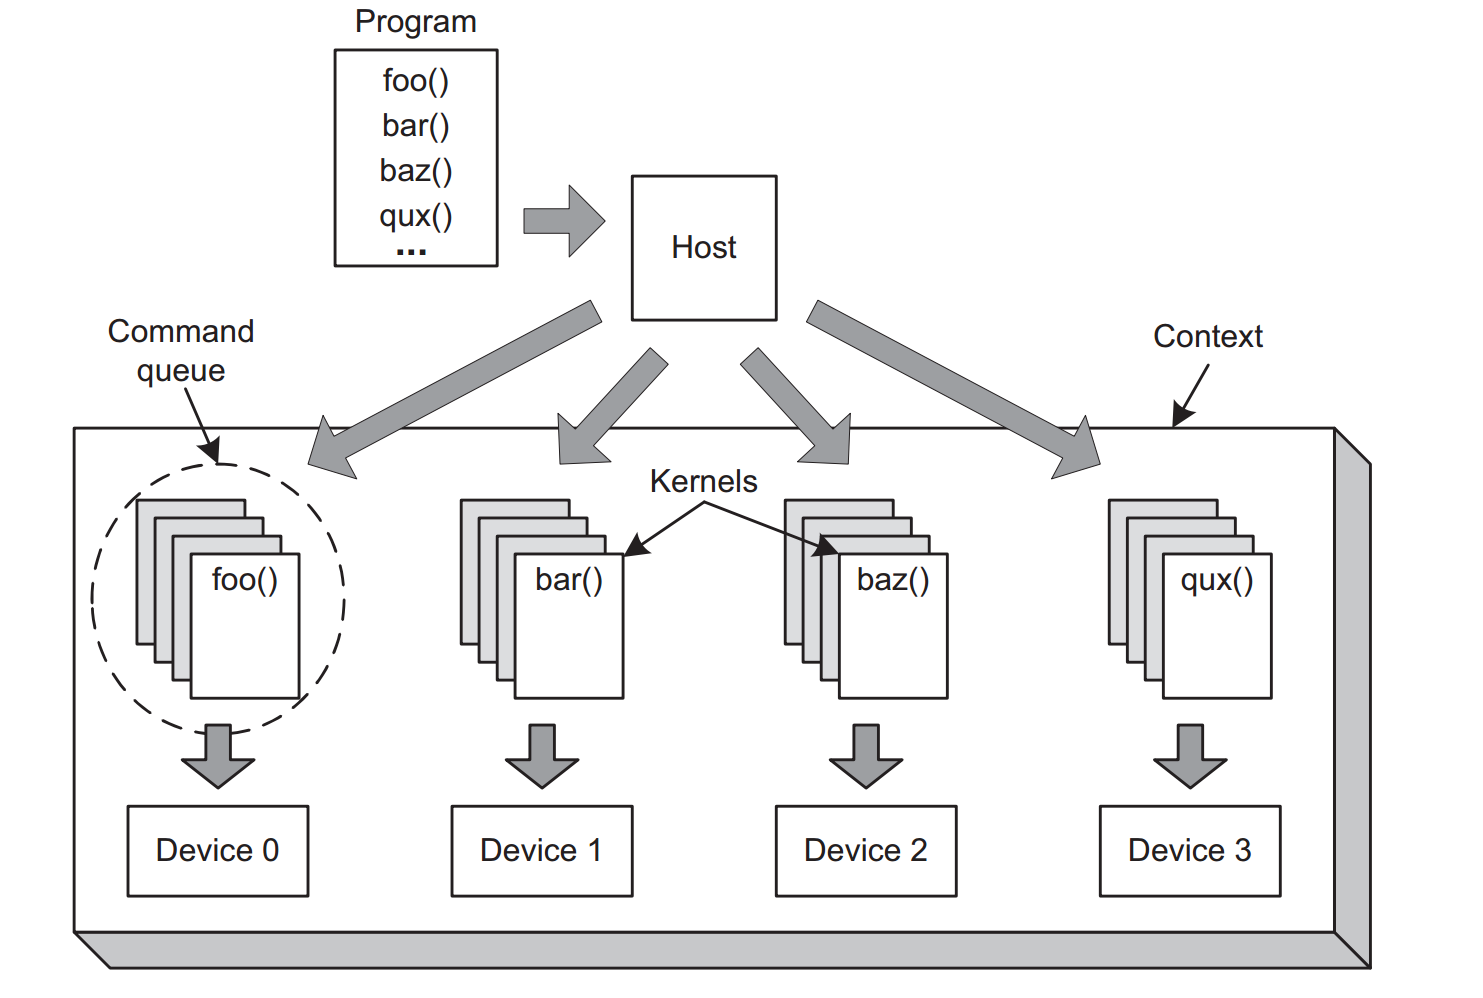
\includegraphics[width=12cm]{./images/OpenCAL-CL/kernelDistribution}
    \caption{General structure of a OpenCL program, from \emph{OpenCL
        in Action: How to accelerate graphics and computations},
      Matthew Scarpino, Manning Pubblication, ISBN-13:
      860-1400825129.}
    \label{fig:GeneralStructure}
  \end{center}
\end{figure}

In order to better understand how OpenCAL-CL works, it is necessary to
introduce some OpenCL concepts. In OpenCL, data exchange and kernels
execution are managed thanks to an OpenCL \emph{context}. In
particular, the host application links kernels into one or more
containers, called \emph{programs}. The program therefore connects
kernels with the data to be processed and dispatches them to a special
OpenCL structure called \emph{command queue}. This is necessary
because only enqueued kernel are actually executed. Figure
\ref{fig:GeneralStructure} shows the general structure of an OpenCL
application. Context contains all the devices, command queues and
kernels, each device has its own command queue and each command queue
contains the kernels to be executed on the corresponding device.

In the following sections, both device- and host-side OpenCAL-CL
programming are briefly introduced. The 2D version of OpenCAL-CL is
here considered for the proposed examples and discussions. However,
note that the same considerantion also holds for the 3D and also any
data type, constant and function presented for the 2D case have a 3D
equivalent.


\subsection{OpenCAL-CL device-side Programming}

As stated above, functions that can be executed on an OpenCL compliant
device are called kernels. In order to explain ho to write an
OpenCAL-CL based kernel, let us condider the example in Listing
\ref{lst:OpenCAL-CL-kernel}.

First of all, the \verb'calcl2D.h' header file must be included (line
1). Accordingly to OpenCL, each kernel definition must start with the
\verb'__kernel' keyword (line 8). However, differently to OpenCL,
where a kernel can have no parameters, each OpenCAL-CL kernel must
have at least the \verb'__CALCL_MODEL_2D' parameter. Actually, it is a
macro-like C object defining a list of pre-fixed typed parameters,
needed to let the kernel to know any data about the CA model, like
subates and neighbourhood, beside others. Kenerls can also take other
parameters, as in the example in Listing
\ref{lst:Another-OpenCAL-CL-kernel}. In the specific case, the
\verb'Pepsilon' parameter is allocated into the compliant device's
global memory. It is also possible to allocate kernel parameters in
the faster local memory, which is shared by threads belonging to the
same work group, by means of the OpenCL \verb'__local'
keyyword. Eventually, kernel parameters can also be private to the
current thread by means of the \verb'__private' keyword, as shown in
Listing \ref{lst:kernel-private-parameter}. The same holds for
variables defined inside the kernel body where the above cited
\verb'__global', \verb'__local' and \verb'_private' memory level
qualifiers can be used. Note that both kernel parameters and variables
declared vithout any memory level qualifier are implicitly considered
as private, as in the case of variables at lines 15 and 16 of Listing
\ref{lst:OpenCAL-CL-kernel}.

\begin{lstlisting}[float,floatplacement=H, label=lst:OpenCAL-CL-kernel, caption=Example of OpenCAL-CL kernel.] 
  #include <OpenCAL-CL/calcl2D.h>

  // Define handles to CA substates
  //...
  #define Z 4
  #define H 5

  __kernel void calcl_kernel_example (__CALCL_MODEL_2D)
  {
    // Prevent the execution of more threads than the CA dimension
    calclThreadCheck2D();
    //...

    // Get the cell coordinates back
    CALint i = calclGlobalRow();
    CALint j = calclGlobalColumn();
    //...

    // Set a new value for the substate
    // whose handle is defined by H.
    // Please, note the usage of the
    // MODEL_2D macro-like object
    calclSet2Dr(MODEL_2D, H, i, j, h_next);
    //...
  }
\end{lstlisting}

The \verb'calclThreadCheck2D()' function in Listing
\ref{lst:OpenCAL-CL-kernel} must be the first to be called into the
kernel, as it prevents the execution of a number of threads exceeding
the number of CA cells\footnote{In fact, OpenCAL-CL adopts the
  one-thread/one-cell policy.} (Listing \ref{lst:OpenCAL-CL-kernel},
line 11). If the active cells optimization is considered, the
\verb'calclActiveThreadCheck2D()' must be called instead of
\verb'calclThreadCheck2D()', to prevent the execution of a number of
threads exceeding the number of CA cells actually involved in
computation. The \verb'calclGlobalRow()' and
\verb'calclGlobalColumn()' functions (Listing
\ref{lst:OpenCAL-CL-kernel}, lines 15-16) are used to get the global
cell coordinates within the cellular space. OpenCAL-CL also provides
the \verb'calclLocalRow()' and \verb'calclLocalColumn()' functions,
which provide the cell coordinates with respect the cellular space
subset assigned to the OpenCL (local) work group. Oter functions that
can be used within an OpenCAL-CL kernel are listed in Table
\ref{tab:kernel-utility-function}.


\begin{table}
  \centering
  \begin{footnotesize}
  \begin{tabular}{l|l}
    \hline
    Function & Brief description\\
    \hline
    \hline
    calclGetRows()                 & Get the number of CA rows \\
    calclGetColumns()              & Get the number of CA columns \\
    calclGetSlices()               & Get the number of CA columns \\
    calclGlobalRow()               & Get the row coordinate for the current cell \\
    calclGlobalColumn()            & Get the column coordinate for the current cell \\
    calclGlobalSlice()             & Get the slice coordinate for the current cell \\
    calclgGetByteSubstatesNum()    & Get the number of substates of \verb'CALbyte' type \\
    calclGetIntSubstatesNum()      & Get the number of substates of \verb'CALint' type \\
    calclGetRealSubstatesNum()     & Get the number of substates of \verb'CALreal' type \\
    calclGetCurrentByteSubstates() & Get a pointer to the set of current layer of \verb'CALbyte' substates \\ 
    calclGetCurrentIntSubstates()  & Get a pointer to the set of current layer of \verb'CALint' substates \\ 
    calclGetCurrentRealSubstates() & Get a pointer to the set of current layer of \verb'CALreal' substates \\ 
    calclGetNextByteSubstates()    & Get a pointer to the set of next layer of \verb'CALbyte' substates \\ 
    calclGetNextIntSubstates()     & Get a pointer to the set of next layer of \verb'CALint' substates \\  
    calclGetNnextRealSubstates()   & Get a pointer to the set of next layer of \verb'CALreal' substates \\ 
    %% calclGetActiveCells()          & Get a pointer to the set of active cells \\
    %% calclGetActiveCellsNum()       & Get the number of active cells \\
    %% calclGetActiveCellsFlags()     & Get a pointer to the set of active cells flags \\
    calclGetNeighborhood()         & Get a pointer to the set of neighboring cells \\
    calclGetNeighborhoodID()       & Get the neighbourhood ID (e.g. von Neumann, Moore, etc.) \\
    calclGetNeighborhoodSize()     & Get the neighbourhood size \\
    calclGetBoundaryCondition()    & Get the boundary condition (simple or cyclic) \\
    calclRunStop()                 & Stops the simulation \\
    \hline
    \end{tabular}
    \end{footnotesize}
  \caption{Some OpenCAL-CL utility kernel functions.}
  \label{tab:kernel-utility-function}
\end{table} 

Note that, functions that in OpenCAL were requiring a pointer to a CA
object, here take the \verb'MODEL_2D' macro-like C object in its place
(line 23), which implicitly defines a list of prefixed parameters
needed by the function. Moreover, substates are accessed by means of
numerical handles (cf. Listing \ref{lst:OpenCAL-CL-kernel}, line 23),
which have to be previously defined into the kernel (Listing
\ref{lst:OpenCAL-CL-kernel}, line 6). The criterion to be adopted is
very simple. Handels are zero-based IDs. Zero is used to link the
first host-side substate, i.e. the first substate added to the
host-side CA, one is used to link the second substate added to the
host-side CA, and so on.

\begin{lstlisting}[float,floatplacement=H, label=lst:Another-OpenCAL-CL-kernel, caption={Another example of OpenCAL-CL kernel, with an additional global parameter.}] 
  #include <calcl2D.h>
  //...
    
  __kernel void another_calcl_kernel_example (__CALCL_MODEL_2D, __global CALParameterr * Pepsilon)
  {
    
    //...
  }
\end{lstlisting}

\begin{lstlisting}[float,floatplacement=H, label=lst:kernel-private-parameter, caption={Another example of OpenCAL-CL kernel, with an additional private parameter.}] 
  #include <calcl2D.h>
  //...
    
  __kernel void another_calcl_kernel_example (__CALCL_MODEL_2D, __private CALParameterr Pepsilon)
  {
    
    //...
  }
\end{lstlisting}



%% \subsection{Selection of the OpenCL compliant device}
\subsection{OpenCAL-CL host-side Programming}

An OpenCAL-CL host application is typically
subdivided in the following parts:
\begin{itemize}
\item Definition of the host-side CA model;
\item Selection of the OpenCL compliant device;
\item Definition of the device-side CA model;
\item Kernels reading, compilation and enqueuing;
\item Simulation execution on the previously selected compliant
  device.
\end{itemize}

All these phases are described below.

\subsubsection{Definition of the host-side CA model}

The OpenCAL-CL host-side CA definition does not differ from what done
for the cases of OpenCAL (cf. Chapter \ref{ch:opencal}). Indeed, in
Listing \ref{lst:host-side-application}, a 2D host-side CA object is
declared by using the \verb'CALModel2D' OpenCAL data type (line 4),
and then initialized by means of the \verb'calCADef2D()' function
(line 11), exactly as in the serial version of OpenCAL. Note that the
\verb'calcl2D.h' OpenCAL-CL specific header file is included at line
1. It, in turn, includes the \verb'cal2D' header, so that it is
possible to use OpenCAL's data types and functions from an OpenCAL-CL
host application.

\begin{lstlisting}[float,floatplacement=H, label=lst:host-side-application, caption={An example of OpenCAL-CL host-side application.}] 
  #include <OpenCAL-CL/calcl2D.h>
  //...

  struct CALModel2D* hostCA;
  //...
  
  int main(int argc, char** argv)
  {
    //...

    hostCA = calCADef2D(ROWS, COLS, CAL_VON_NEUMANN_NEIGHBORHOOD_2D, CAL_SPACE_TOROIDAL, CAL_OPT_ACTIVE_CELLS);
    //...
        
  }
\end{lstlisting}


\subsubsection{Selection of the OpenCL compliant device}

OpenCAL-CL provides the \verb'CALOpenCL' structure that, together with
other utility functions, considerably simplifies platform, device, and
context management with respect to the native OpenCL API. Listing
\ref{lst:CALOpenCL} shows how to select a compliant device in
OpenCAL-CL.

\begin{lstlisting}[float,floatplacement=H, label=lst:CALOpenCL, caption=Access to platform and devices.]
  #include <OpenCAL-CL/calcl2D.h>
  //...

  int main (int argc, char** argv)
  {
    // Initilize a pointer to the CALCLManager structure
    CALCLManager * calcl_manager = calclCreateManager ();

    // get all available platforms
    calclInitializePlatforms ( calcl_manager );

    // Initialize the devices
    calclInitializeDevices ( calcl_manager );

    // Uncomment if platforms and devices are unknown
    //calclGetPlatformAndDeviceFromStdIn();

    // get the first device on the first platform
    // this call is unnecessary if calclGetPlatformsAndDeviceFromStandardInput() is used
    CALCLdevice device = calclGetDevice ( calcl_manager , 0, 0 );

    // create a context
    CALCLcontext context = calclCreateContext ( &device , 1 );

    // ...
  }
\end{lstlisting}

The \verb'calcl2D.h' header file is included at line 1. Line 7
declares a pointer to \verb'CALCLManager', and initializes it through
the \verb'calclCreateManager()' function. This object, named
\verb'calcl_manager', is then used as parameter for the
\verb'calclInitializePlatforms()' function (line 10), which fills the
object with the platforms available on the machine. Line 13 calls the
\verb'calclInitializeDevices()' function, that initializes the
available devices, while line 20 selects one of them for kernel
execution. Specifically, an object of type \verb'CALCLdevice' is
declared ad initialized by the function \verb'calclGetDevice()'. This
latter takes a pointer to a \verb'CALOpenCL' object as first
parameter, while the second and third parameters specify the platform
and device to be selected, respectively. Since both platforms and
devices are identified by a 0-based index\footnote{In OpenCAL-CL
  platforms and devices are stored in a matrix where rows represent
  platforms and columns devices. Thus, to choose which platform and
  device to use for the computation, it is necessary to specify their
  indexes within the matrix. For example, at lines 15, we chose the
  platform number 0 and the device number 0. If we have a system with
  3 NVIDIA GPUs and 3 AMD GPUs, the library will have a $2 \times 3$
  size matrix, where 2 are the vendors (i.e., the platforms NVIDIA and
  AMD) and 3 are the GPUs for each platforms. If we want to run the
  program using the third AMD GPU, we can specify 1 and 2 as
  indices.}, statement at line 20 selects the first device belonging
to the first platform (e.g. a GTX 980 belonging to the NVIDIA CUDA
platform). If system's platforms and devices are unknown, the
\verb'calclGetPlatformAndDeviceFromStdIn()' function can be used
alternatively to \verb'calclGetDevice()'. It prints all the available
platforms and devices to standard outpunt and permits for their
interactive selection from standard input. Eventually, line 23 creates
an OpenCL context, based on the device previously selected. For this
porpose, an object of \verb'CALCLcontext' type is declared and defined
by means of the \verb'calclCreateContext()' function.


\subsubsection{Definition of the device-side CA model}

OpenCAL-CL allows for having a counterpart of the host-side CA to
device-side. Such a device-side CA is declared as a
\verb'CALCLModel2D' object and, beside managing all the CA components
device-side, it also provides simulation execution features. Note
that, this is a main difference with respect to OpenCAL serial
version, where the simulation execution is managed by a complementary
object, specifically of type \verb'CALRun2D'. To initialize the
device-side CA object, the \verb'calclCADef2D' function can be used
(cf. Listing \ref{lst:calclCADef2D}). The first parameter is a pointer
to a \verb'CALModel2D', defined host side as in the case of the serial
implementation of OpenCAL (cf. Chapter \ref{ch:opencal}). The second
one is an OpenCL context, as well as the third and fourth parameters
are an OpenCL program and compliant device, respectively.

%% The device-side CA object permits to equeue the defined kernels

\begin{lstlisting}[float,floatplacement=H, label=lst:calclCADef2D, caption=The calclCADef2D data structure., numbers=none]
  CALCLModel2D * calclCADef2D(
                   struct CALModel2D * host-model,
                   CALCLcontext context,
                   CALCLprogram program,
                   CALCLdevice device
  )
\end{lstlisting}


\subsubsection{Kernels reading, compilation and enqueuing}

After the compliant device has been selected and elementary processes
(and possibly other functions) implemented as kernels, these latter
can automatically be read and compiled through the
\verb'calclLoadProgram2D()' function (cf. Listing
\ref{lst:calclLoadProgram}). It takes both the context and device, and
also the paths to directories containing the user defined kernels and
related headers (if any) as parameters, and returns an OpenCL
program\footnote{\texttt{CALCLprogram} redefines the
  \texttt{cl\_program} OpenCL type.}. All the files in the kernel
source directory are automatically considered, indipendently from
their name. Note that, since kernel headers are optional, the last
parameter can be \verb'NULL'.

\begin{lstlisting}[float,floatplacement=H, label=lst:calclLoadProgram, caption={The calclLoadProgramLib function. It loads and compiles kernels by returning an OpenCL program.}, numbers=none]
  CALCLprogram calclLoadProgram2D (
    CALCLcontext context ,
    CALCLdevice device ,
    char * kernel_source_directory ,
    char * kernel_include_directory
  )
\end{lstlisting}

Once compiled and grouped into an OpenCL program, kernels can be
extracted in order to be attached to a command queue for
execution. Specifically, the \verb'calclGetKernelFromProgram()'
function extracts a kernel from an OpenCL program, taking a pointer to
the program and the kernel name (cf. Listing
\ref{lst:calclGetKernelFromProgram}).

\begin{lstlisting}[float,floatplacement=H, label=lst:calclGetKernelFromProgram, caption={The calclGetKernelFromProgram kernel extraction function}., numbers=none]
  CALCLkernel calclGetKernelFromProgram (
    CALCLprogram * program,
    char * kernelName 
  )
\end{lstlisting}

The function \verb'calclAddElementaryProcess2D' adds a new kernel to
the execution queue (cf. Listing
\ref{lst:calclAddElementaryProcess2D}), in a transparent manner to the
user. The function takes both a pointer to host and device CA as
parameter and also a pointer to an OpenCL kernel.

\begin{lstlisting}[float,floatplacement=TH, label=lst:calclAddElementaryProcess2D, caption=The calclAddElementaryProcess2D function., numbers=none]
  void calclAddElementaryProcess2D(
               CALCLModel2D * deviceCA,
               struct CALModel2D * hostCA,
               CALCLkernel * kernel
  );
\end{lstlisting}

Note that, if the kernel to be added has one or more parameters
(beside the mandatory \verb'__CALCL_MODEL_2D' one), they must be
passed to the device-side application. Passing a parameter to a
kernels is a operation which depends on how the parameter is declared:
if as a pointer or not.

Let as consider the example in Listing
\ref{lst:Another-OpenCAL-CL-kernel}, where a parameter is declared as
a pointer to be stored into the device's global memory. A double step
procedure must be used in this case. Fist, the
\verb'calclCreateBuffer()' function must be called. It takes the
OpenCL context, the address of the host parameter to be passed to the
kernel, and the dimension of the host parameter type, and returns an
object of type \verb'CALCLmem', which is a buffer containing the value
of the host-side parameter. This buffer is therefore used by the
\verb'calclSetKernelArg2D()' function, which actually perform the data
transmission to the device. It takes the kernel to which send the
parameter, the parameter position within the kernel parameter list (0
for the first one after the mandatory \verb'__CALCL_MODEL_2D'
parameter, 1 for the second, and so on), the \verb'CALCLmem'
dimension, and the address of the buffer containing the value for the
kernel parameter (cf. Listing \ref{lst:calclKernelParameters}).

At the contrary, if the kernel parameter is not declared as a pointer,
like in the example in Listing \ref{lst:kernel-private-parameter}, the
above double step process is no longer necessary, since it is
sufficient to call the \verb'calclSetKernelArg2D()' by specifying as
third parameter the dimension of the actual type of the variable to be
passed to the kernel. 

%% calclSetKernelArg2D(&kernel_elem_proc_flow_computation, 1, sizeof(CALParameterr), &P.r);

\begin{lstlisting}[float,floatplacement=H, label=lst:calclSetKernelArg2D, caption=The calclSetKernelArg2D() function., numbers=none]
  calclSetKernelArg2D(&kernel_elem_proc_flow_computation,
                      1,
                      sizeof(CALParameterr),
                      &P.r
  );
\end{lstlisting}


\begin{lstlisting}[float,floatplacement=H, label=lst:calclKernelParameters, caption=Passing parametrs to kernel.]
  #include <OpenCAL-CL/calcl2D.h>
  //...
  
  struct sciddicaTParameters {
    CALParameterr epsilon;
    //...
  } P;

  //...
  
  int main(int argc, char** argv)
  {
    //...
    CALCLmem bufferEpsilonParameter;
    //...

    bufferEpsilonParameter = calclCreateBuffer(context, &P.epsilon, sizeof(CALParameterr));
    calclSetKernelArg2D(&kernel_elem_proc_flow_computation, 0, sizeof(CALCLmem), &bufferEpsilonParameter);    
    //...
  }
\end{lstlisting}


\subsubsection{Simulation execution on the compliant device}

The \verb'calclRun()' function (cf. Listing \ref{lst:calclRun2D}) runs
the CA simulation by executing all the defined kernels on the selected
compliant device. The first two parameters are pointers to a device
and host CA, respectively, while the last two are the initial and
final step for the simulation execution. If the last parameter is set
to \verb'CAL_RUN_LOOP', simulation never ends. In this case, to stop
the simulation, the user must define a stop condition criterion
through the \verb'calclAddStopConditionFunc2D()' function
(cf. \ref{lst:calclAddStopConditionFunc2D}). Note that, since the stop
condition must be evaluated host side, it must be implemented as a
kernel. For this reason, the tird parameter is a pointer to an OpenCL
kernel. Other kernel can be registered to the device-side CA. Table
\ref{tab:XXX} list all the register functions to the device-side CA.


\begin{table}
  \centering
  \begin{footnotesize}
  \begin{tabular}{l|l}
    \hline
    Function & Brief description\\
    \hline
    \hline
    XXX()                 & XXX \\
    \hline
    \end{tabular}
    \end{footnotesize}
  \caption{}
  \label{tab:XXX}
\end{table} 



\begin{lstlisting}[float,floatplacement=H, label=lst:calclRun2D, caption=The calclRun2D function., numbers=none]
  void calclRun2D(CALCLModel2D* deviceCA,
                  struct CALModel2D * hostCA,
                  unsigned int initialStep,
                  unsigned maxStep
  );
\end{lstlisting}


\begin{lstlisting}[float,floatplacement=H, label=lst:calclAddStopConditionFunc2D, caption=The calclAddStopConditionFunc2D function., numbers=none]
  void calclAddStopConditionFunc2D(
                 CALCLModel2D * deviceCA,
                 struct CALModel2D * hostCA,
                 CALCLkernel * kernel
  );
\end{lstlisting}


\section{Conway's Game of Life with OpenCAL-CL}
 
As already reported in \ref{sec:cal_life}, to introduce how to develop
a CA model with OpenCAL-CL we can start by implementing Conway’s Game
of Life and specifically its host application part, which is shown in
Listing \ref{lst:calcl_life}. In order to use OpenCAL-CL, some header
files are included (lines 3-8) and, in particular, the OpenCAL library
and the OpenCAL-CL library. The OpenCAL library inclusion is necessary
to define the CA object (line 46) and the related substates (line
49). The \verb'cal2DIO.h' header file (line 4) provides some basic
input/output functions for reading/writing substates from/to file. To
run the application with OpenCAL-CL, all the necessary objects have to
be declared (line 27-31): specifically, the \verb'CALOpenCL' structure
(line 27), the \verb'CALCLcontext', the \verb'CALCLdevice', the
\verb'CALCLprogram' and the \verb'CALCLToolkit2D'. To create and
initialize these variables we need to call the function
\verb'calclCreateManager' that creates the CALOpenCL structure, the
functions \verb|calclInitializePlatforms| and
\verb|calclInitializeDevices| that initialize all the platforms and
devices on the available machine and the \verb'calclGetDevice()'
function, which will return the device where elementary process are
computed by choosing the \verb'platformNum' and \verb'deviceNum'
integers(line 24-25). Moreover, two important functions are here
considered: \verb'calclcreateContext' and
\verb'calclLoadProgram2D'. The first returns the context
(see \ref{sec:opencalclstructure}), while the second builds all kernels inside
the path specified by \verb'kernelSrc'(line 15) including the files
specified by \verb'kernelInc'(line 16), and returns a program
containing all the compiled kernels.

The definition and declaration of the model (line 46) has the same code
that we discussed in \ref{sec:cal_life}, and includes all the information
to create the model, to create and initialize substates (line 49-52) and 
to set a initial configuration (line 55-59).

\lstinputlisting[label=lst:calcl_life, caption=An OpenCAL-CL
  implementation of the Conway's game of
  Life.]{../opencal/OpenCAL-CL/examples/calcl_life/source/life.c}
	
Although the OpenCAL-CL library uses the same functions of the OpenCAL
library to create the model and the substates, the execution of the
elementary processes is quite different. As known, our elementary
processes are implemented on GPU side through kernels, so we need to
manage the transfer of memory between host and device sides and to
decide which and when run the kernels. In a classical OpenCL
application, it's not trivial to handle all these issues. For this
reason, in OpenCAL-CL we decided to introduce an intermediate object
(\verb'CALCLToolkit') that hides to the user the memory management and
handles the compiled chosen kernels. The user must only initialize the
\verb'CALCLToolkit' structure(line 62) and choose which kernel he/she
wants to execute by the function \verb'calclGetKernelFromProgram'
specifying the program and kernel names. Once kernels are chosen to be
executed, the user must only call the function
\verb'calclAddElementaryProcessKernel2D' (line 71) that adds the
specific kernel elementary process inside the \verb'CALCLToolkit'
structure. Finally, to run the simulation, the user must call the
function \verb'calclRun2D' specifying the initial and final step.

Below is reported the device-side code of Conway's Game of Life.  In
this application, we have only one elementary process, defined as a
kernel called \verb'life_transition_function'. The OpenCAL-CL library
will launch exactly a number of threads equal to the entire cellular
space, structured like a matrix. In this way, every cell can perform
in parallel its own computation. To access to the indexes of the cell
the user must call the function \verb'getRow' and \verb'getCol'
line(14-15). Furthermore, the user can use the function
\verb'get_columns' and \verb'get_rows' (line 17-18) to retrieve the
dimensions of the cellular space.  In the specific case of the Game of
Life, we used the \verb'calGet2Di' function to get the central cell’s
value of the substate Q (remember that the central cell is identified
by the coordinates (i, j)), the \verb'calGetX2Di' function to retrieve
the value of the n-th neighbour’s substate Q, and the \verb'calSet2Di'
function to update the value of the substate Q for the central cell.

\lstinputlisting[label=lst:calcl_life, caption=An OpenCAL-CL kernel
  to implement the Conway's game of Life elementary
  process.]{../opencal/OpenCAL-CL/examples/calcl_life/kernel/source/life.cl}

\section{SciddicaT in OpenCAL-CL}

\section{A three-dimensional example}

\section{Combining OpenCAL-OMP and OpenCAL-GL, and Global Functions}

As for OpenCAL, it is possible to exploit OpenCAL-GL to have a simple
visualization system by adding few lines of code to your
application. Combining OpenCAL-CL and OpenCAL-GL does not differ from
what we have done in Section \ref{sec:combining_gl} for OpenCAL and
OpenCAL-GL. Therefore, please refer to this section for major
details.

Similarly, you can use the same global reduction functions
described in Section \ref{sec:redution} also in OpenCAL-CL.  Please
refer to that section for further details.
